\documentclass[11pt]{article}
\usepackage[utf8]{inputenc}
\usepackage{scrextend}
\usepackage[portuges]{babel}
\usepackage{natbib}
\usepackage{graphicx}
\usepackage{listings}
\usepackage{color}
\usepackage{titling}

\definecolor{dkgreen}{rgb}{0,0.6,0}
\definecolor{gray}{rgb}{0.5,0.5,0.5}
\definecolor{mauve}{rgb}{0.58,0,0.82}
\renewcommand{\lstlistingname}{Excerto}
\lstset{frame=tb,
  language=Java,
  aboveskip=3mm,
  belowskip=3mm,
  showstringspaces=false,
  columns=flexible,
  basicstyle={\small\ttfamily},
  numbers=none,
  numberstyle=\tiny\color{gray},
  keywordstyle=\color{blue},
  commentstyle=\color{dkgreen},
  stringstyle=\color{mauve},
  breaklines=true,
  breakatwhitespace=true,
  tabsize=3
}

% \code para fonte console
\newcommand{\code}{\texttt}

\title{
    \Large{Trabalho Prático de Sistemas Distribuídos} \\
    \Large{Universidade do Minho}
    \vspace{-10pt}}
\author{\small André Gonçalo Castro Peixoto, A82260\\
        \small Henrique José Carvalho Faria, A82200\\
        \small Luís Filipe da Costa Cunha, A83099\\
        \small Miguel Ângelo Moreira Ramos Brandão, A82349
        \vspace{-20pt}}
\date{}


\begin{document}
% begin Página inicial

\setlength{\droptitle}{-60pt}
\maketitle

%\begin{figure}[h!]
%\centering
%
\includegraphics[scale=0.3]{Logo.png}
%\end{figure}

% end Página inicial

\section{Introdução}

O principal objetivo deste trabalho foi desenvolver um serviço de alocação de servidores na Internet e de contabilização do custo incorrido pelos utilizadores.

Cada utilizador pode reservar um servidor fazendo um pedido ou indo a leilão. Quando reserva a pedido, o cliente fica com um servidor, que permanece exclusivo até ser libertado. Adicionalmente, é cobrado um preço correspondente ao tempo utilizado.

Quando o utilizador reserva em leilão, este propõe o preço que se dispõe a pagar para reservar um servidor de determinado tipo. Depois disso, só lhe é atribuído um servidor quando o preço horário proposto for o maior entre todos os licitantes para esse tipo de servidor. Além disto, as reservas em leilão, podem ser canceladas pela nuvem de forma a satisfazer uma reserva a pedido quando não existam outros servidores disponíveis do tipo pretendido.
%----------------------------------------------------------

\section{Funcionalidades}
Como proposto, o software que realizamos suporta as seguintes funcionalidades:
\begin{enumerate}
    \item \textbf{Autenticação e registo de utilizador: dado email e palavra-passe.} Quando um utilizador deseja interagir com o serviço, o servidor estabelece uma conexão e autentica-o;
    \item \textbf{Reservar um servidor a pedido.} Um utilizador autenticado pode pedir a reserva de um servidor de um determinado tipo (pelo preço nominal);
    \item \textbf{Reservar uma instância em leilão.} Um utilizador autenticado pode pedir a reserva de um servidor de um determinado tipo indicando o preço horário que se dispõe a pagar;
    \item \textbf{Libertar um servidor.} Um utilizador autenticado pode terminar uma reserva de um servidor que anteriormente lhe foi concedida;
    \item \textbf{Consultar a sua conta corrente.} Um utilizador autenticado consegue consultar o valor em dívida de acordo com a utilização dos recursos da plataforma de computação na nuvem.
    \item Os tipos de servidores disponíveis são fixos e previamente conhecidos;
    \item O número de servidores disponível de cada tipo é fixo e previamente conhecido;
    \item Cada tipo de servidor tem uma identificação e preço nominal fixos e previamente conhecidos;
    \item A operação de reserva de um servidor a pedido espera até que seja concedida e devolve um identificador da reserva que mais tarde é utilizado para a terminar;
    \item Em caso de indisponibilidade de servidores do tipo pedido, podem ser canceladas reservas concedidas em leilão para obter o servidor pretendido;
    \item A libertação de uma reserva concedida a pedido pode ser feita pelo utilizador a quem foi concedida utilizando o identificador correspondente. O servidor considera a instância libertada como disponível para futura reserva;
    \item A operação de reserva de um servidor em leilão indica qual o preço pretendido, espera até que seja concedida e devolve um identificador da reserva, que mais tarde é utilizado para a terminar;
    \item Caso haja várias operações de reserva em leilão para um tipo de servidor que passa a estar disponível, é considerada aquela que ofereça o valor mais alto.
    \item Caso uma reserva concedida em leilão seja cancelada pela nuvem, o utilizador é avisado utilizando o identificador correspondente;
    \item A libertação de uma reserva concedida em leilão pode ser feita pelo utilizador a quem foi concedida utilizando o identificador correspondente. O servidor considerar a instância libertada como disponível para futura reserva.
\end{enumerate}

\noindent
\textbf{Cliente:} temos uma interface "cliente" que permite ao utilizador usar e usufruir de todas as funcionalidades anteriores. Esta interface usa threads e sockets TCP, tal como foi realizado nas aulas práticas ao longo do semestre.
\\
\\
\noindent
\textbf{Servidor:} também criámos um servidor com threads e sockets TCP, que suporta todas as funcionalidades anteriores, para além de receber conexões e inputs dos utilizadores e responder com a informação adequada a cada pedido. Esta troca de informação é feita através de linhas de texto e cada thread escreve em apenas um socket.
Existem dez tipos de servidores: somas, substrações, divisões, multiplicações, texto, excel, word, paint, leitura e programação.

%----------------------------------------------------------
\section{Código}

\subsection{Classe \code{Cliente}}

Esta é a classe que define um cliente do serviço, ou seja, é a classe a partir da qual é criada cada instância \emph{cliente}. Para cada cliente são guardados o seu ID único, a sua password, as suas reservas ativas e a sua dívida, bem como uma \code{ReentrantLock} associada a este. Esta classe define alguns dos habituais \emph{getters}, \emph{setters} e outros métodos tradicionais de POO, bem como alguns métodos mais particulares:

\begin{labeling}{\code{removeReserva}}
    \item [\code{addReserva}] dados uma reserva e o seu número, adiciona a reserva à lista das reservas do cliente
    \item [\code{removeReserva}] dado o número de uma reserva, remove-a da lista de reservas do cliente
    \item [\code{growDivida}] dado um \code{double}, adiciona-o ao montante de dívida atual do cliente
\end{labeling}

\subsection{Classe \code{ClienteServidor}}
Esta classe contém única e exclusivamente a \code{main} dedicada à execução do terminal de acesso do cliente. A \code{main} inicia um socket conectado ao servidor, criando de seguida um \code{BufferedReader} para ler o que o for escrito pelo servidor (a interface de texto) e um \code{PrintWriter} para interagir com o servidor, assegurando a conexão e a interação entre servidor e cliente até ao cliente escrever \emph{fim}, instruindo a função a terminar a conexão.

\subsection{Classe \code{GestorReservas}}
Esta classe contém apenas um \code{int nReserva} e uma \code{ReentrantLock}, com o respetivo construtor, um método para incrementar em '1' o \code{nReserva} e o seu respetivo \emph{get}. A função desta classe é armazenar o número de reserva atual, pelo que só terá uma instância, que pode ser entendida como uma variável global \emph{thread safe} e será utilizada para serem atribuídos os números de reserva às reservas dos servidores.

\subsection{Classe \code{Informacao}}
As instâncias desta classe definem um tipo de servidores. São guardados o nome do servidor, o número de servidores disponíveis para reserva normal e também para reserva por licitação, o número de servidores reservados no momento, o preço, uma lista com as reservas em vigor e outra com as licitações em espera.

São implementados os seguintes métodos mais importantes:

\begin{labeling}{\code{isPossible}}
    \item [\code{isPossible}] este método é responsável por verificar na lista de servidores ocupados se existem servidores de leilão que ainda não tenham sido reservados. Assim que  encontrar um, devolve o seu ID de reserva para poder ser reservado pelo cliente que o quer.
    \item [\code{mudaDono}] dado o número de uma reserva, o ID do novo cliente e a lista de clientes da ”empresa”, move-se a reserva do servidor do cliente do momento para o novo cliente,  aumentando-se a dívida do cliente que estava a utilizar o servidor.
    
\end{labeling}

\subsection{Classe \code{Reserva}}
A classe \code{Reserva} é responsável por guardar o intervalo de tempo associado à reserva de um servidor, que é utilizado posteriormente para calcular a dívida do cliente correspondente. O seu método mais importante é o seguinte:

\begin{labeling}{\code{getDivida}}
    \item [\code{getDivida}] este método calcula o preço de aluguer de um determinado servidor, consoante o intervalo de tempo pelo qual é reservado.
\end{labeling}

\subsection{Classe \code{Servidor}}

Nesta classe, definimos os constituintes básicos de um servidor deste serviço. Estes elementos básicos são: o tipo de aluguer (leilão ou reserva), o tipo de reserva e o ID de cliente. Ao contrário de outras classes, a classe \code{Servidor} não contem métodos adicionais, para além dos seus \emph{getters}, \emph{setters} e construtores.

\subsection{Classe \code{Servidores}}

Esta classe guarda todos os servidores (e inicializa-os), assim como todos os clientes do sistema. É aqui que gerimos a conexão entre estes duas entidades, através da utilização de um \code{ServerSocket} (que fica à escuta de novos clientes) e o uso de várias threads (uma para cada cliente).
A classe servidores só contém uma função \code{main}.

\subsection{Classe \code{ThreadAutentica}}

A classe \code{ThreadAutentica} corresponde à execução de uma thread no servidor, que conduz o utilizador por todas as funcionalidades do sistema, utilizando buffers (reader e writer) para determinar as ações que o utilizador pretende efetuar. As várias funcionalidades que o sistema proporciona a cada cliente estão no método \code{run}, tais como: alugar servidor, consultar a dívida, etc...
%----------------------------------------------------------

\section{Operação do programa}
Antes de concluir, demonstramos aqui alguns \emph{screenshots} de apenas algumas funcionalidades da aplicação, de maneira a ilustrar um pouco toda esta informação textual:

\begin{figure}[h]
    \centering
    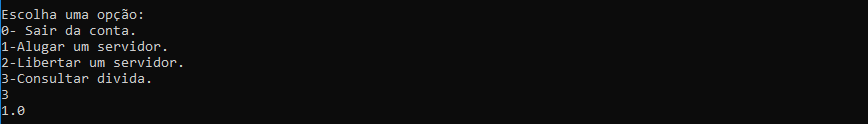
\includegraphics[width=\textwidth]{Consultar_Divida.png}
    \caption{Consultar dívida}
    \label{fig:consultar_divida}
\end{figure}

\begin{figure}[h]
    \centering
    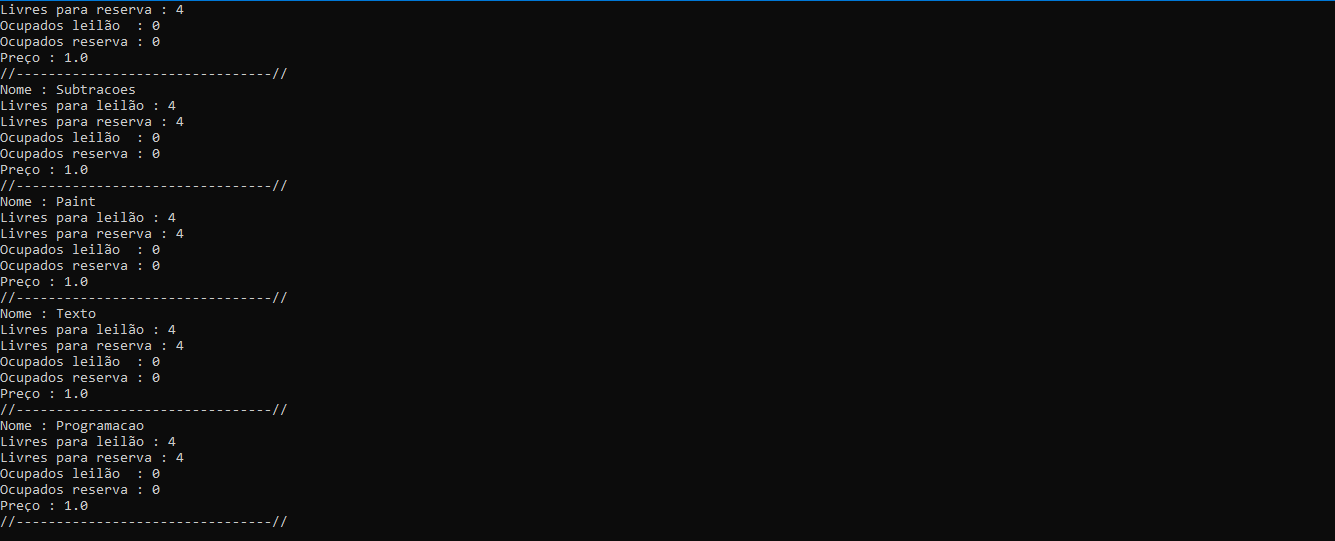
\includegraphics[width=\textwidth]{Alugar_Servidor_parte_2.png}
    \caption{Alguns servidores para exemplo}
    \label{fig:exemplo_tipos_servidores}
\end{figure}

\begin{figure}[h]
    \centering
    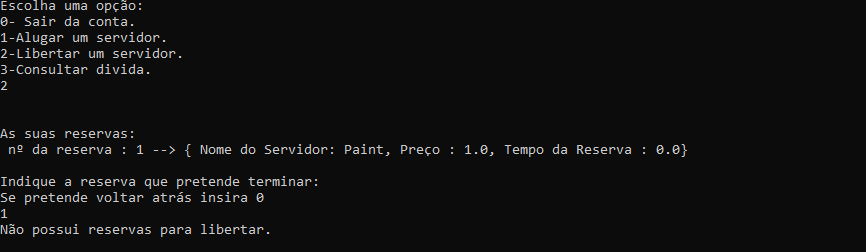
\includegraphics[width=\textwidth]{Libertar_Servidor.png}
    \caption{Libertar servidor}
    \label{fig:libertar_servidor}
\end{figure}

%----------------------------------------------------------
\newpage
\section{Conclusão}

Com a realização deste trabalho, consolidámos os nossos conhecimentos relativos à disciplina de Sistemas Distribuídos, tais como: criação de threads em Java, partilha de objetos entre threads, exclusão mútua na execução de secções críticas, evitar deadlocks, uso de locks para exclusão mútua, conexão via TCP, uso de delimitação orientada a linha de texto, implementação de servidores sequenciais, implementação de servidores multi-threaded sem estado partilhado entre clientes, implementação de servidores multi-threaded (com estado partilhado entre clientes) e controlo de concorrência. Fazendo uma apreciação final do nosso projeto, estamos confiantes que conseguimos alcançar os objetivos propostos para o desenvolver do nosso software de alocação de servidores na nuvem, pois cremos que atingimos as funcionalidades requeridas pelos professores com uma estrutura de código bastante otimizada.

\end{document}
